% !TEX root = ../agglo_clust_review.tex
% 
\begin{figure}
\centering
        \begin{subfigure}[t]{0.46 \linewidth}
        \centering
        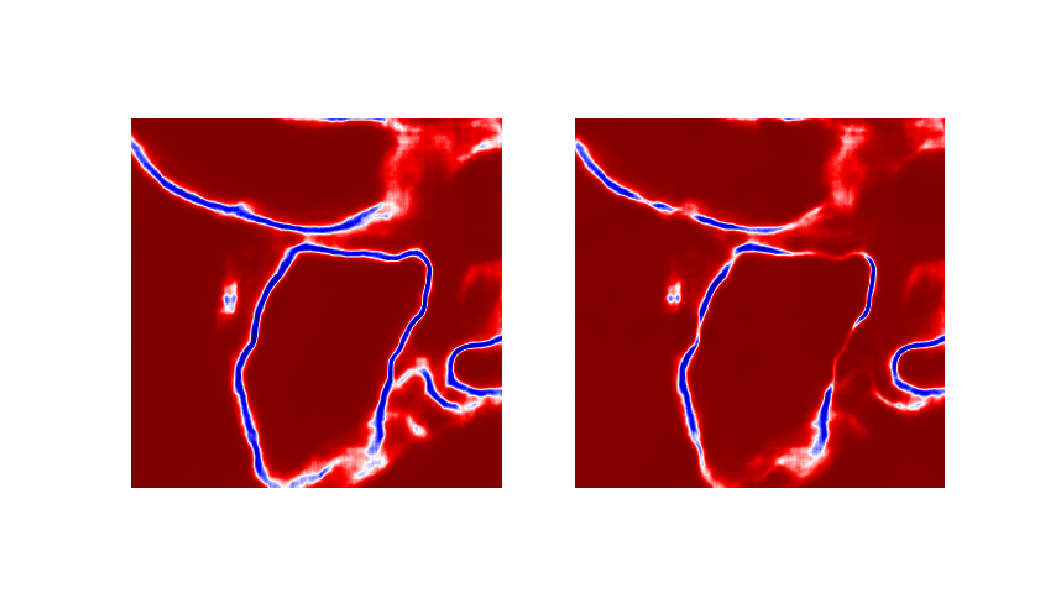
\includegraphics[width=0.98\textwidth,trim=4.4in 1.2in 0.in 0.05in,clip]{figs/noisy_affs_merge.pdf}
        % \caption{Thresholding of local boundary maps ~(THRESH)} \label{fig:thresh}
    \end{subfigure}%
    \begin{subfigure}[t]{0.46 \linewidth}
        \centering
        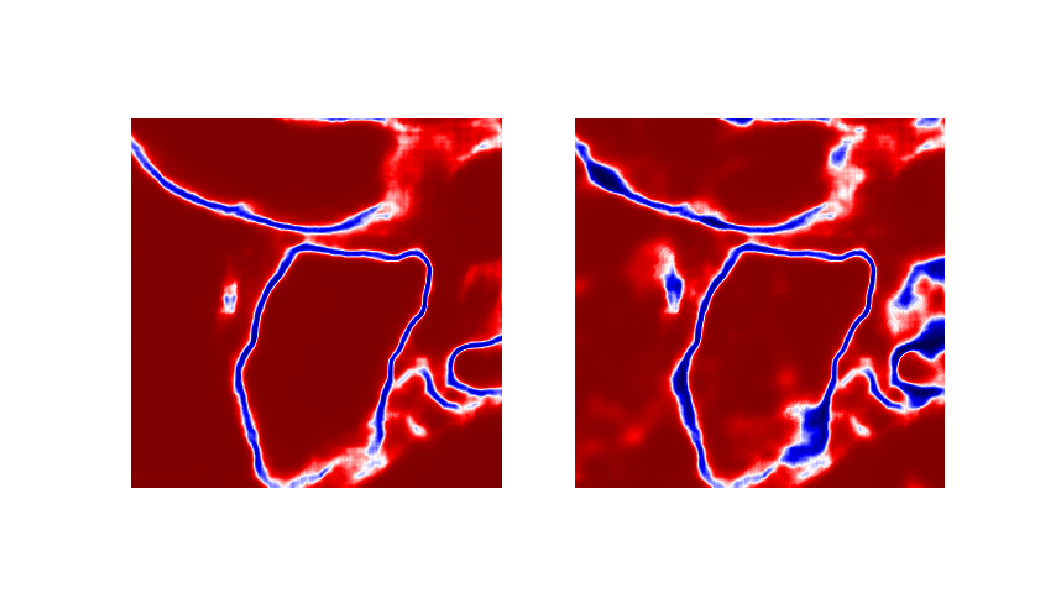
\includegraphics[width=0.98\textwidth,trim=4.4in 1.2in 0.in 0.05in,clip]{figs/noisy_affs_split.pdf}
        % \caption{Watershed, seeded at local minima of the smoothed input map~(WS)} \label{fig:ws}
    \end{subfigure}\hspace{0.5cm}%
    \caption{Noisy affinities \TODO{Left: clean affinities. Right: divide image in two triangles and show split and merge simultaneously}}
    % \label{fig:isbi-examples}
\end{figure}% 

\subsection{Noise experiments}
\begin{itemize}
    \item In this section we will quantitatively test the robustness of the unified agglomerative clustering algorithm by adding noise to the edge weights of the graph and see how different choices of update rules compare.
    \item Among the update rules listed in Table \ref{tab:linkage-criteria}, we will focus only on \emph{sum}, \emph{arithmetic mean} and \emph{absolute maximum}, since they achieved the best scores in the results presented in Sec. \ref{sec:exp_first_comparison}. Before to present the results shown in Fig. \ref{fig:noise_merge} and \ref{fig:noise_split}, we will first introduce the type of noise that was added to the edge weights.
\item In the set of analyzed experiments, edge weights are estimated \UPDATE{by using a CNN that predicts pairwise interactions between pixels in the image/volume}. Fig. \ref{fig:noisy_affinities}a illustrates the predictions of the CNN for neighboring pixels in the horizontal direction of Define Perlin/opensimplex noise
\item Present plots
\item Comment about MC energy
\end{itemize}


\begin{figure}
\centering
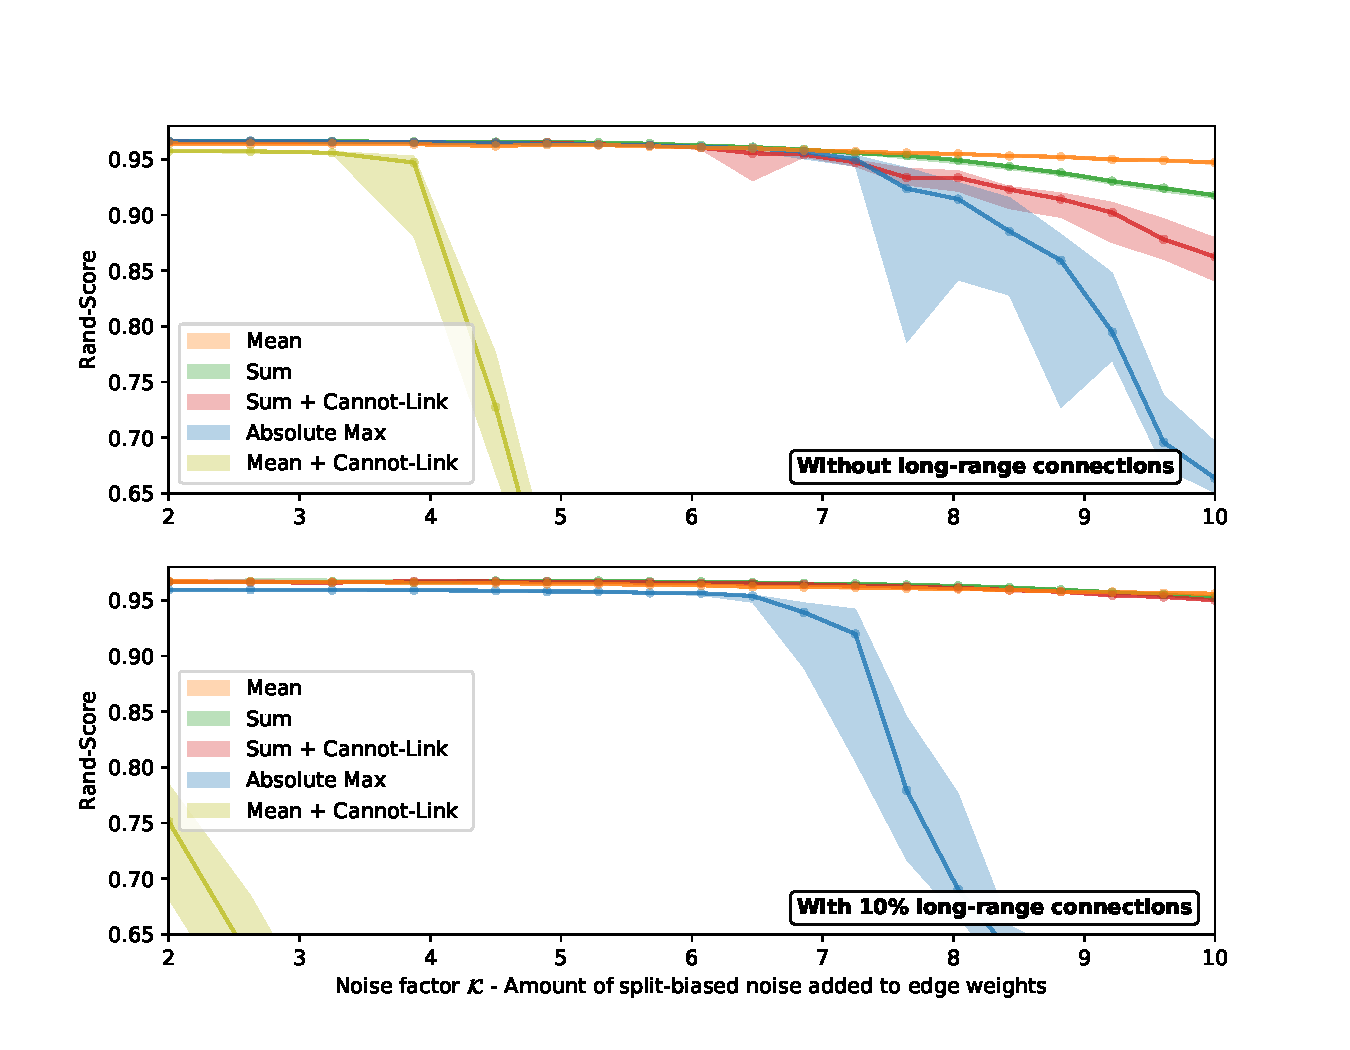
\includegraphics[width=0.50\textwidth,trim=0.27in 0.27in 0.27in 0.27in,clip]{./figs/split_noise.pdf}
\caption{Plot illustrating results with split-biased noise...}\label{fig:noise_split}
\end{figure}


% \begin{figure}
% \centering
% \includegraphics[width=0.50\textwidth,trim=0.27in 0.27in 0.27in 0.27in,clip]{./figs/noisy_affs.pdf}
% \caption{Illustration of noisy affinities}\label{fig:noisy_affinities}
% \end{figure}
